\newpage
\section{Общие сведения о системе}

\subsection{Вход в систему}

Перед началом работы в системе необходимо получить персональный идентификатор пользователя (логин) и пароль у администратора.

\begin{vnim}
 Персональный идентификатор и пароль предназначены для индивидуального доступа в систему. Никогда не сообщайте их третьим лицам!
\end{vnim}
 
Для того чтобы начать работать с Системой администрирования ЛПУ, необходимо войти в нее, используя персональный идентификатор и пароль. Процедура входа в систему называется \dm{авторизацией}. \label{auth}

\begin{figure}[ht]\centering
 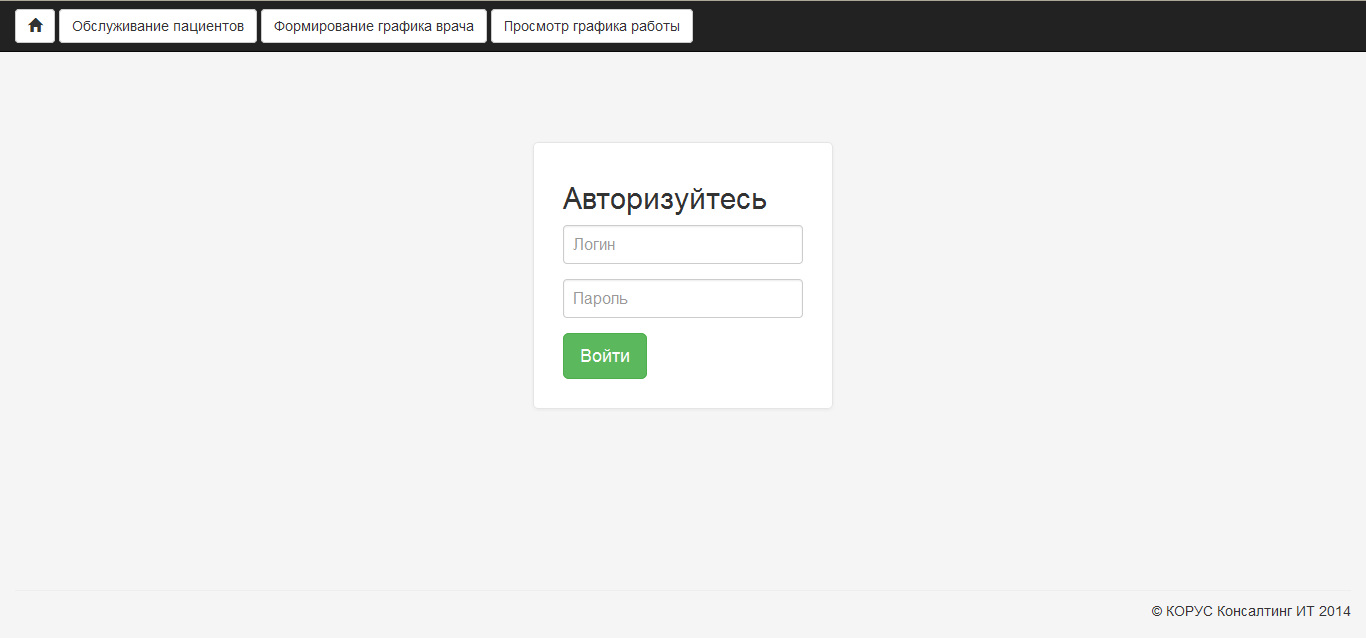
\includegraphics[width = 1\textwidth ,keepaspectratio]{gen_login}
 \caption{Форма авторизации пользователя}
 \label{img_gen_login}
\end{figure} 

Доступ к системе можно получить следующими способами:
\begin{itemize}
 \item Запустить приложение с помощью ярлыка на рабочем столе.
 \item Открыть любой из доступных Web-браузеров (Internet Explore, Firefox, Opera, Chrome и др.) и в адресной строке ввести адрес сервера, полученный у администратора системы.
\end{itemize}

После выполнения любого из описанных действий откроется форма авторизации (Рисунок \ref{img_gen_login}), где следует ввести идентификатор пользователя, пароль и нажать кнопку \btn{Войти}.

В случае успешной авторизации откроется главная страница системы (Рисунок \ref{img_gen_main}).

\begin{figure}[ht]\centering
 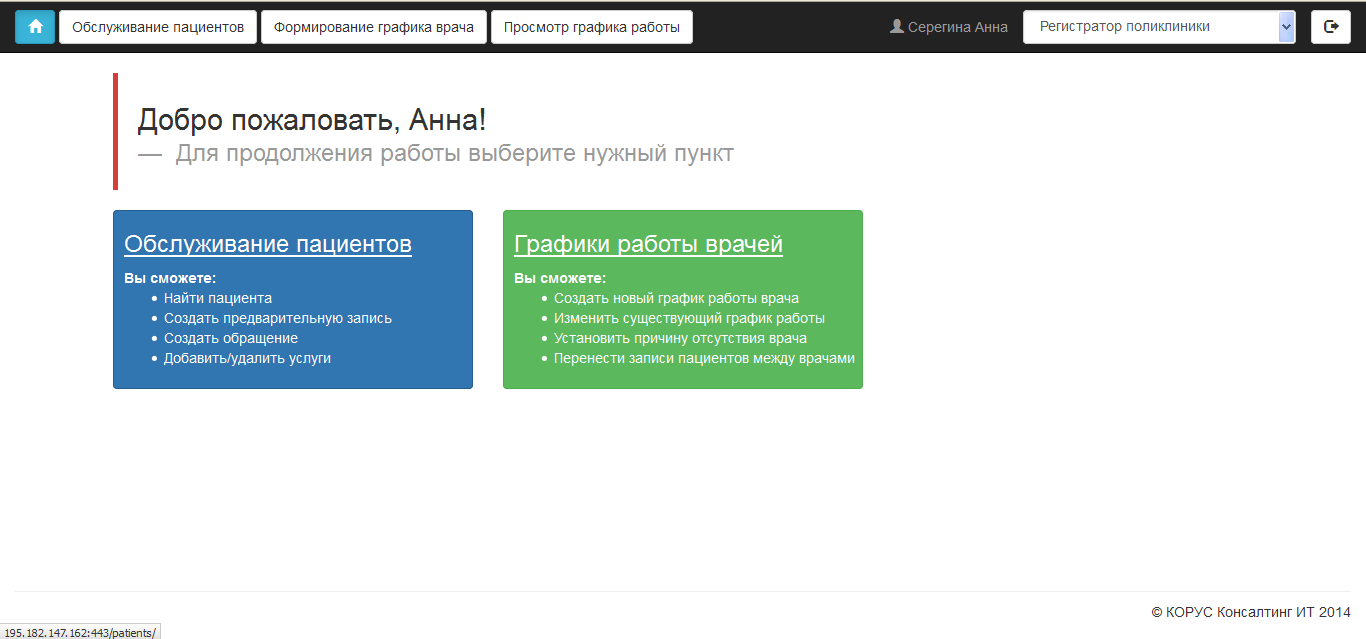
\includegraphics[width = 1\textwidth ,keepaspectratio]{gen_main}
 \caption{Главная страница системы}
 \label{img_gen_main}
\end{figure} 

Если в процессе авторизации возникла какая-либо ошибка, сообщение появится над полем для ввода логина (Рисунок \ref{img_gen_lfail}).

В случае возникновения ошибки «Неверная пара логин/пароль» необходимо:
\begin{enumerate}
 \item Проверить правильность введенного идентификатора пользователя;
 \item Проверить правильность введенного адреса для подключения (если вводился вручную);
 \item Проверить язык ввода;
 \item Проверить состояние клавиши \keys{CapsLock} на клавиатуре и выключить ее при необходимости;
 \item Если в пароле присутствуют цифры, проверить состояние клавиши \keys{NumLock}, включить ее при необходимости;
 \item Повторить попытку авторизации.
\end{enumerate}
 
Если проблема не была решена, нужно обратиться к администратору системы для проверки идентификационных данных.

\begin{figure}[ht]\centering
 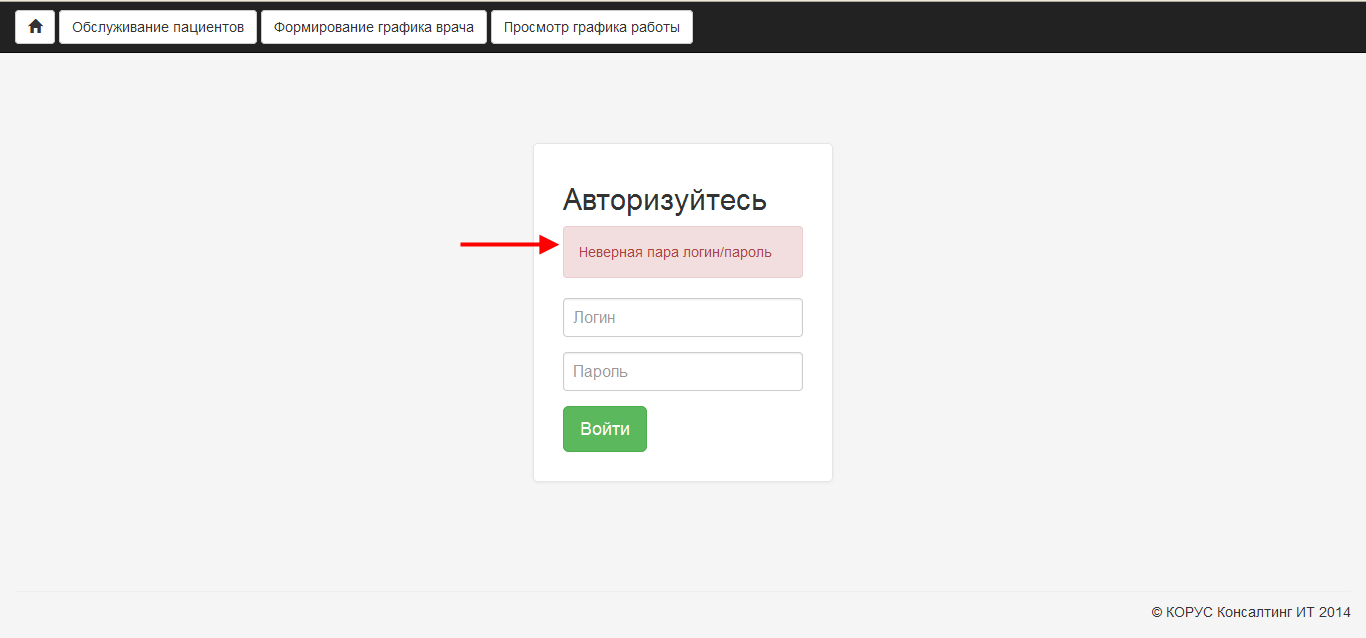
\includegraphics[width = 1\textwidth ,keepaspectratio]{gen_lfail}
 \caption{Ошибка авторизации}
 \label{img_gen_lfail}
\end{figure} 

\subsection{Завершение работы}

После завершения работы, необходимо выйти из системы. Для этого нужно нажать кнопку 
\includegraphics{exit} в правом верхнем углу страницы. Будет осуществлен выход из системы и возврат на страницу авторизации. Если требуется войти в систему под другим именем пользователя, следует пройти процедуру авторизации с новыми идентификационными данными. Если работа с системой завершена, можно закрыть Web-браузер, нажав на кнопку \btn{x} в правом верхнем углу окна или выбрав в главном меню пункт \mm{Файл \str Выход}.

\subsection{Основные принципы работы}

Система администрирования ЛПУ (или система) работает через Web-интерфейс и не требует установки на клиентской рабочей станции никакого дополнительного программного обеспечения. Единственным обязательным условием является наличие установленного Web-браузера, который, как правило, включен по умолчанию при установке любой операционной системы.

Вся работа в системе производится в окне Web-браузера. В верхней части каждой страницы находится панель управления (Рисунок \ref{img_gen_main}).

В левой ее части находятся список доступных подсистем. При нажатии на кнопку с названием подсистемы осуществляется переход на главную страницу выбранной подсистемы. При нажатии на кнопку 
\includegraphics{home} выполняется переход на главную страницу системы.

В правой части панели управления находятся следующие кнопки:
\begin{itemize}
 \item Кнопка 
\includegraphics{help}  вызывает справку по основным управляющим элементам текущей страницы.
 \item Кнопка 
\includegraphics{exit}  позволяет выйти из системы.
\end{itemize}

\begin{prim}
 После авторизации в системе возможно одновременное открытие нескольких страниц системы. Страницы могут быть открыты в отдельных окнах или вкладках. Для открытия страницы в новой вкладке или новом окне можно воспользоваться контекстным меню или колесом прокрутки мыши.
\end{prim}

\subsubsection{Работа со справкой}

Кнопка 
\includegraphics{help}  находится на панели управления в правом верхнем углу любой страницы Системы администрирования ЛПУ. При нажатии на нее появляется окно подсказки, последовательно описывающее назначение основных управляющих элементов страницы (Рисунок \ref{img_gen_help}).

\begin{figure}[ht]\centering
 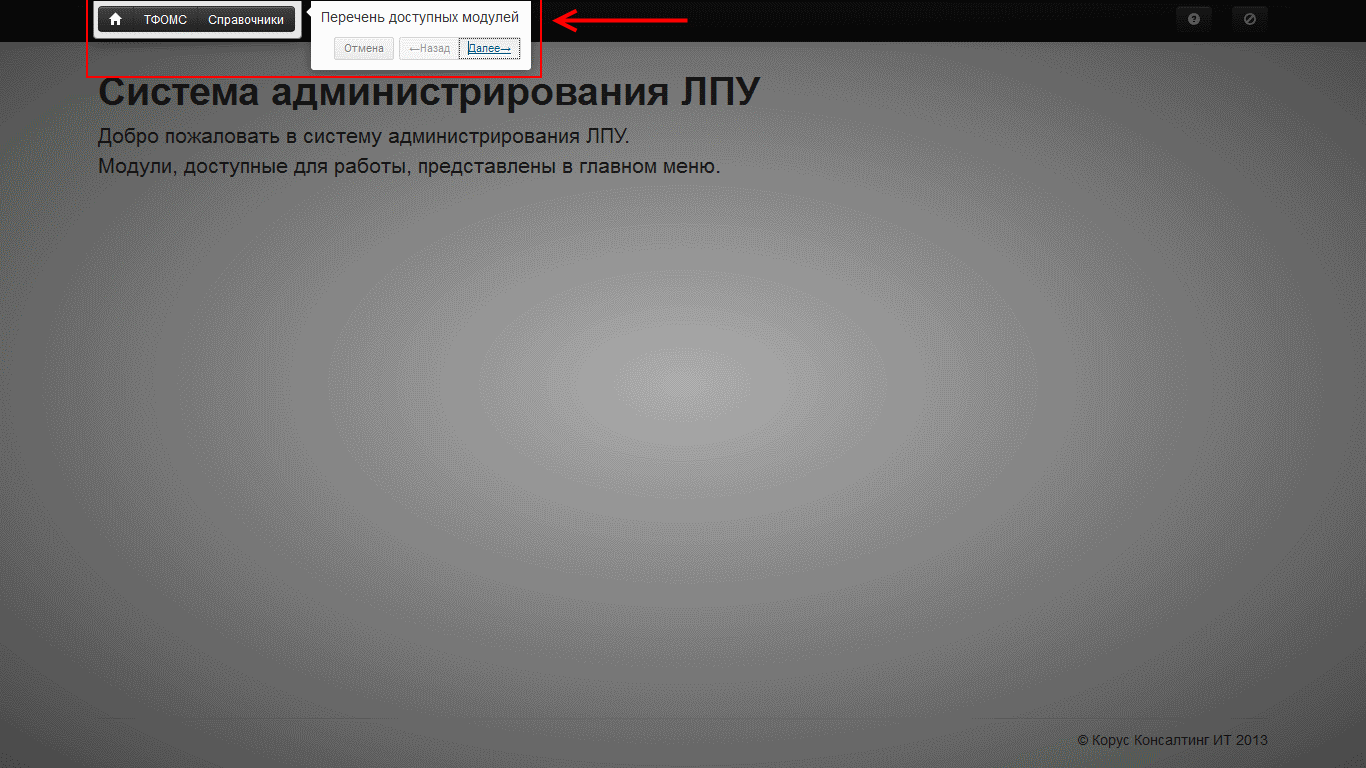
\includegraphics[width = 1\textwidth ,keepaspectratio]{gen_help}
 \caption{Справка по панели управления}
 \label{img_gen_help}
\end{figure} 

Для перехода к следующему элементу необходимо нажать кнопку \btn{Далее $\to$}  в окне подсказки или клавишу \keys{$\to$} на клавиатуре. Окно подсказки переместится к следующему управляющему элементу страницы и отобразит подсказку по нему. Если был достигнут последний управляющий элемент страницы, то окно подсказки закрывается.

Для возврата к предыдущему управляющему элементу нужно нажать кнопку \btn{$\gets$ Назад}  или клавишу \keys{$\gets$} на клавиатуре.

При нажатии на кнопку \btn{Отмена} окно подсказки закрывается.
